\documentclass[compress]{beamer}
\usepackage[
    title={Parallel Matrix Multiplication},
    event={Progetto fine corso SCPA},
    author={MC, LF},
    longauthor={Matteo Conti, Luca Falasca},
    email={},
    institute={SCPA 2023-2024},
    longinstitute={Universita' degli Studi di Roma Tor Vergata},
]{unislides}
\usepackage{graphicx} % Required for inserting images
\usepackage{minted}
\usepackage{algorithm}
\usepackage{hyperref}
\usepackage{adjustbox}
\usepackage{svg}
\svgsetup{inkscapelatex=false}

\begin{document}

\begin{frame}[plain]
    \titlepage
\end{frame}

%---------------------INTRODUZIONE---------------------
\section{Introduzione}

\subsection{Descrizione del problema}
\begin{frame}{\secname \text{ }- \subsecname\ }
    Il progetto verte sull'implementazione di un nucleo di calcolo per effettuare il prodotto tra due matrici dense, definito come:
    \begin{Definition}
        \begin{equation}
            \label{eq:ce_ue}
            C = C + A\cdot B
        \end{equation}
    \end{Definition}
    dove $A$, $B$ e $C$ sono matrici di dimensioni $M\times K$, $K\times N$ ed $M\times N$ rispettivamente, in particolare verranno considerate:
    \begin{itemize}
        \item Matrici quadrate
        \item Matrici rettangolari con $M,N>>K$ con $K=\{32, 64, 128, 156\}$
    \end{itemize}
\end{frame}

\subsection{Obiettivi}
\begin{frame}{\secname \text{ }- \subsecname\ }
    Verranno analizzate le prestazioni di tre differenti implementazioni del prodotto, in particolare:
    \begin{columns}
        \column{0.5\textwidth}
            \begin{minipage}[b]{1\textwidth}
                \begin{itemize}
                    \item MPI, utilizzando il paradigma SIMD per la parallelizzazione su CPU
                    \item CUDA, sfruttando le potenzialità delle GPU per l'accelerazione computazionale
                    \item MPI+CUDA, cercando di combinare i vantaggi delle due precedenti versioni
                \end{itemize}
            \end{minipage}
        \column{0.5\textwidth}
            \begin{minipage}{1\textwidth}
                \begin{adjustbox}{margin=0cm 0cm 0cm 0.2cm, center} % left, bottom, right, top
                    
\includegraphics[width=0.5\textwidth]{resources/cpu_gpu.png}
                \end{adjustbox}
            \end{minipage}
    \end{columns}
\end{frame}

\subsection{Metriche di valutazione}
\begin{frame}{\secname \text{ }- \subsecname\ }
    Per valutare le prestazioni delle soluzioni sviluppate sono stati considerati i FLOPS definiti come:
    \begin{Definition}
        \begin{equation}
            FLOPS = \frac{2MNK}{exec\_time}
        \end{equation}
    \end{Definition}
    \begin{adjustbox}{margin=0cm 0cm 0cm 0.2cm, center} % left, bottom, right, top
        
\includegraphics[width=0.3\textwidth]{resources/performance_icon.png}
    \end{adjustbox}
\end{frame}

\subsection{Raccolta dei dati}
\begin{frame}{\secname \text{ }- \subsecname\ }
    I dati raccolti sono stati ottenuti eseguendo i vari nuclei di calcolo sul server di dipartimento il quale presenta le seguenti specifiche:
    \begin{columns}
        \column{0.5\textwidth}
            \begin{minipage}[b]{1\textwidth}
                \begin{itemize}
                    \item CPU: 2 x Intel Xeon Silver 4210
                    \item Memory: 64 GiB of RAM
                    \item GPU: Nvidia Quadro RTX 5000
                    \item CUDA version: 12.3
                    \item MPI version: 4.1
                \end{itemize}
            \end{minipage}
        \column{0.5\textwidth}
            \begin{minipage}{1\textwidth}
                \begin{adjustbox}{margin=0cm 0cm 0cm 0.6cm, center} % left, bottom, right, top
                    
\includegraphics[width=0.65\textwidth]{resources/pc.png}
                \end{adjustbox}
            \end{minipage}
    \end{columns}
\end{frame}

%---------------------MPI------------------------------
\section{MPI}

\begin{frame}{\secname}
    %TODO
\end{frame}

\subsection{Distribuzione del carico}
\begin{frame}{\secname \text{ }- \subsecname\ }
    %TODO
\end{frame}

\subsection{Riduzione del risultato}
\begin{frame}{\secname \text{ }- \subsecname\ }
    %TODO
\end{frame}

\subsection{Implementazione del prodotto}
\begin{frame}{\secname \text{ }- \subsecname\ }
    %TODO
\end{frame}

\subsubsection*{Implementazione Naive}
\begin{frame}{\secname \text{ }- \subsecname\ \text{ }- \subsubsecname}
    %TODO
\end{frame}

\subsubsection*{Implementazione Column blocked}
\begin{frame}{\secname \text{ }- \subsecname\ \text{ }- \subsubsecname}
    %TODO
\end{frame}

%---------------------CUDA------------------------------
\section{CUDA}

\begin{frame}{\secname}
    %TODO
\end{frame}

\subsection{1 versione}
\begin{frame}{\secname \text{ }- \subsecname\ }
    \begin{columns}
        \column{0.5\textwidth}
            \begin{minipage}{1\textwidth}
                \begin{adjustbox}{margin=0cm 0cm 0cm 0cm, center} % left, bottom, right, top
                    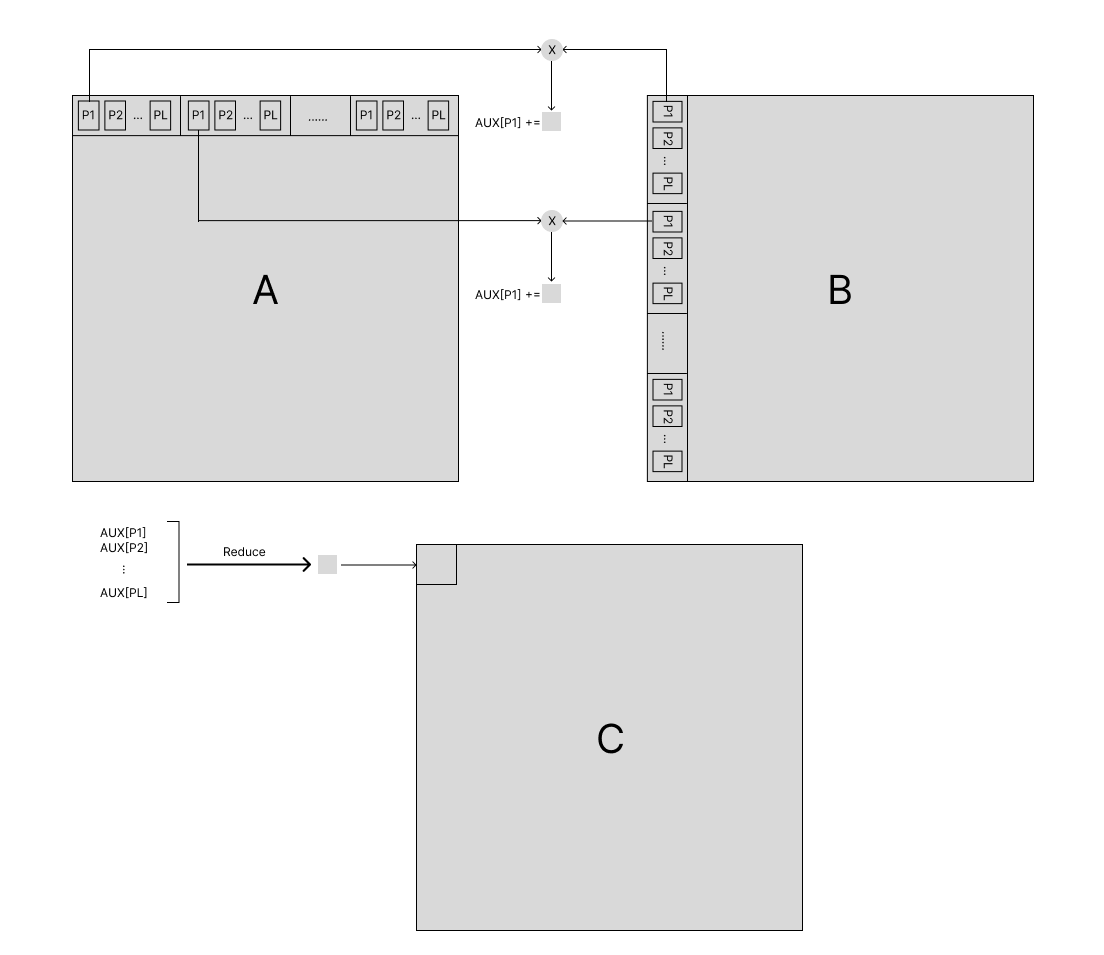
\includegraphics[width=1.2\textwidth]{resources/cuda_scheme_v1.png}
                \end{adjustbox}
            \end{minipage}
        \column{0.5\textwidth}
            \begin{minipage}[b]{1\textwidth}
                \begin{enumerate}
                    \item Divisione della riga di A tra i thread
                    \item Divisione della colonna di B tra i thread
                    \item Calcolo del prodotto per ogni thread
                    \item Memorizzazione dei risultati parziali in shared memory
                    \item Reduce dei risultati parziali
                    \item Scrittura sulla matrice C
                    \item Ripeti per ogni colonna di B
                    \item Ripeti per ogni riga di A
                \end{enumerate}
            \end{minipage}
    \end{columns}
\end{frame}

\begin{frame}{\secname \text{ }- \subsecname\ }
    Nella versione 1 tra il calcolo di una colonna e l'altra, i thread devono sincronizzarsi per poi fare l'operazione di reduce dei risultati parziali. \\ \\
    Questo perchè il vettore in shared memory riesce a contenere solo i risultati della riga di A per 1 colonna di B. \\
    
    \textbf{Soluzione:} \\
    Utilizzare una matrice di shared memory che mantiene i risultati parziali di più colonne per volta.
   \[
        aux = \left[
        \begin{matrix}
        pr_{col_0, t_0} & pr_{col_0, t_2} & ... & pr_{col_0, t_{BD}} \\
        pr_{col_1, t_0} & pr_{col_1, t_2} & ... & pr_{col_1, t_{BD}} \\
        ... & ... & ... & ... \\
        pr_{col_{Q}, t_0} & pr_{col_{Q}, t_2} & ... & pr_{col_{Q}, t_{BD}}
        \end{matrix}\right]
    \]
\end{frame}

\subsection{2 versione}
\begin{frame}{\secname \text{ }- \subsecname\ }
    \begin{columns}
        \column{0.5\textwidth}
        \begin{minipage}[b]{1\textwidth}
            \begin{enumerate}
                \item Divisione della riga di A tra i thread
                \item Divisione delle colonna di B \\tra i thread
                \item Calcolo del prodotto per ogni thread per tutto il gruppo di colonne
                \item Memorizzazione dei risultati parziali in shared memory
                \item Reduce dei risultati parziali 
                \item Scrittura sulla matrice C
                \item Ripeti per ogni gruppo di colonne di B
                \item Ripeti per ogni riga di A
            \end{enumerate}
        \end{minipage}
        \column{0.5\textwidth}
        \begin{minipage}{1.25\textwidth}
            \begin{adjustbox}{margin=0cm 0cm 0cm 0cm, center} % left, bottom, right, top
                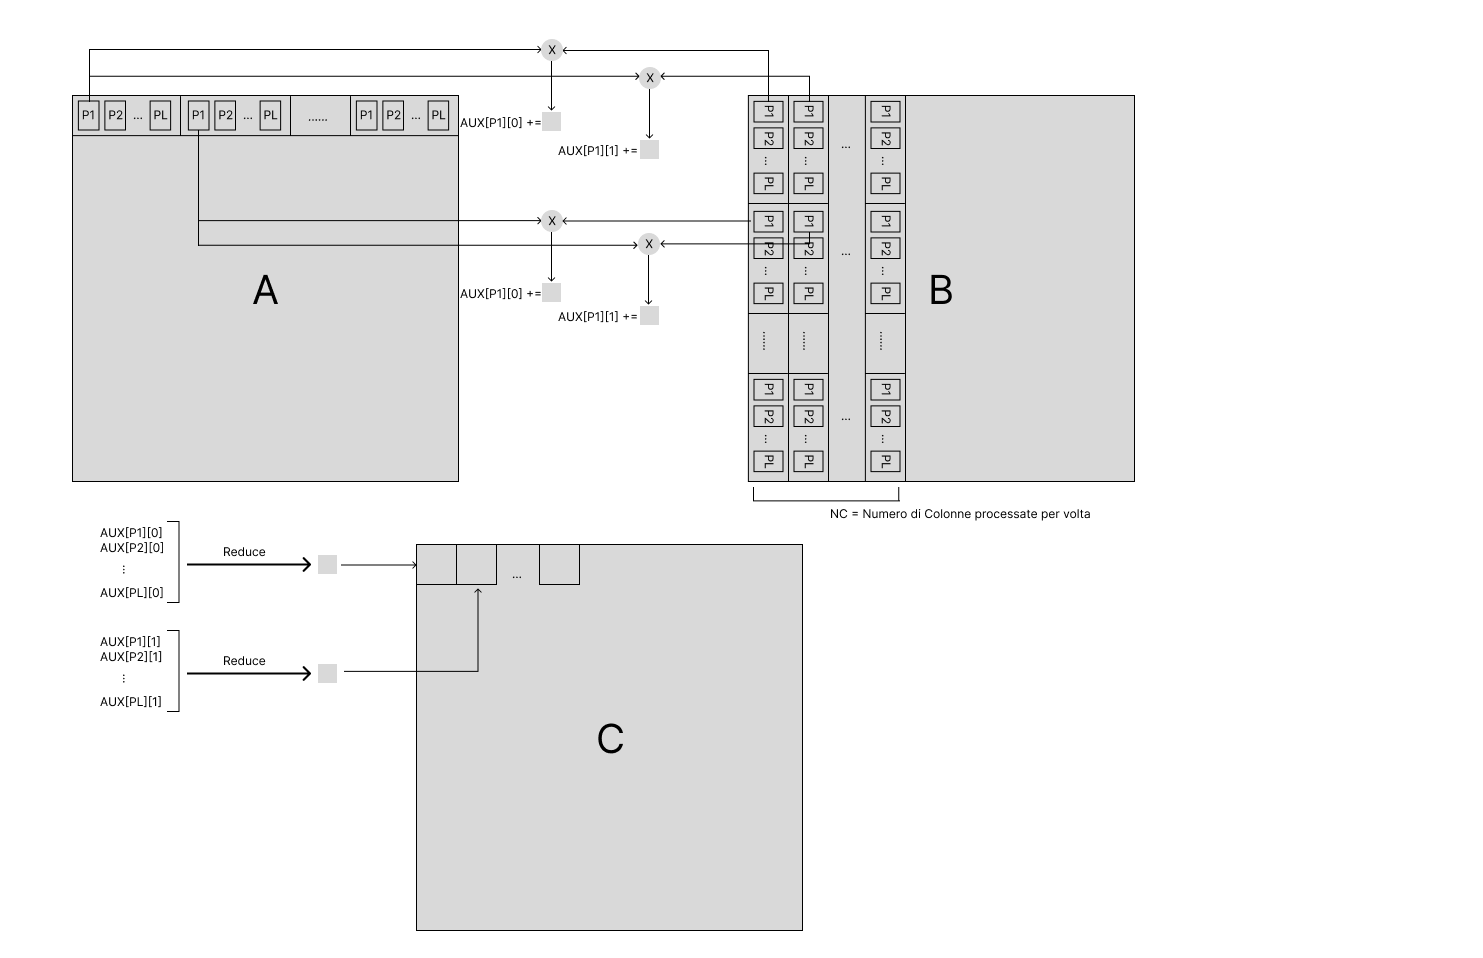
\includegraphics[width=1.2\textwidth]{resources/cuda_scheme_v2.png}
            \end{adjustbox}
        \end{minipage}
        
    \end{columns}
\end{frame}

\begin{frame}{\secname \text{ }- \subsecname\ }
    Nella versione 2 quando si processa il gruppo di colonne, poiché si calcola il risultato parziale di una colonna per volta, per ognuna di esse bisogna riaccedere alla riga della matrice A che è in memoria globale. \\ \\
    
    \textbf{Soluzioni:} \\
    \begin{itemize}
        \item Anziché processare una colonna per volta si processano i primi $BD$ elementi delle Q colonne del gruppo corrente.
        \begin{itemize}
            \item Questo permette di accedere una sola volta alla riga di A.
        \end{itemize}
        \item Mantenere in shared memory parte della colonna A necessario per il calcolo.
        \begin{itemize}
            \item Questo permette di accedere alla memoria globale una sola volta.
            \item Ogni thread accede al proprio elemento della riga di A necessario per il calcolo dalla memoria shared.
        \end{itemize}
    \end{itemize}
\end{frame}

\subsection{3 versione}

\begin{frame}{\secname \text{ }- \subsecname\ }
    \begin{columns}
        \column{0.5\textwidth}
        \begin{minipage}[b]{1\textwidth}
            \begin{enumerate}
                \item Divisione della riga di A tra i thread
                \item Divisione delle colonna di B \\ tra i thread
                \item Memorizzazione della riga parziale di A in shared memory
                \item Calcolo del prodotto per ogni thread per il blocco di righe \\ del gruppo di colonne 
                \begin{itemize}
                    \item ripeti per ogni blocco di \\ righe del gruppo di colonne
                \end{itemize}
                \item Memorizzazione dei risultati parziali in shared memory
                \item Reduce dei risultati parziali 
                \item Scrittura sulla matrice C
                \item Ripeti per ogni gruppo di colonne di B
                \item Ripeti per ogni riga di A
            \end{enumerate}
        \end{minipage}
        \column{0.5\textwidth}
        \begin{minipage}{1.25\textwidth}
            \begin{adjustbox}{margin=0cm 1cm 0cm 0cm, center} % left, bottom, right, top
                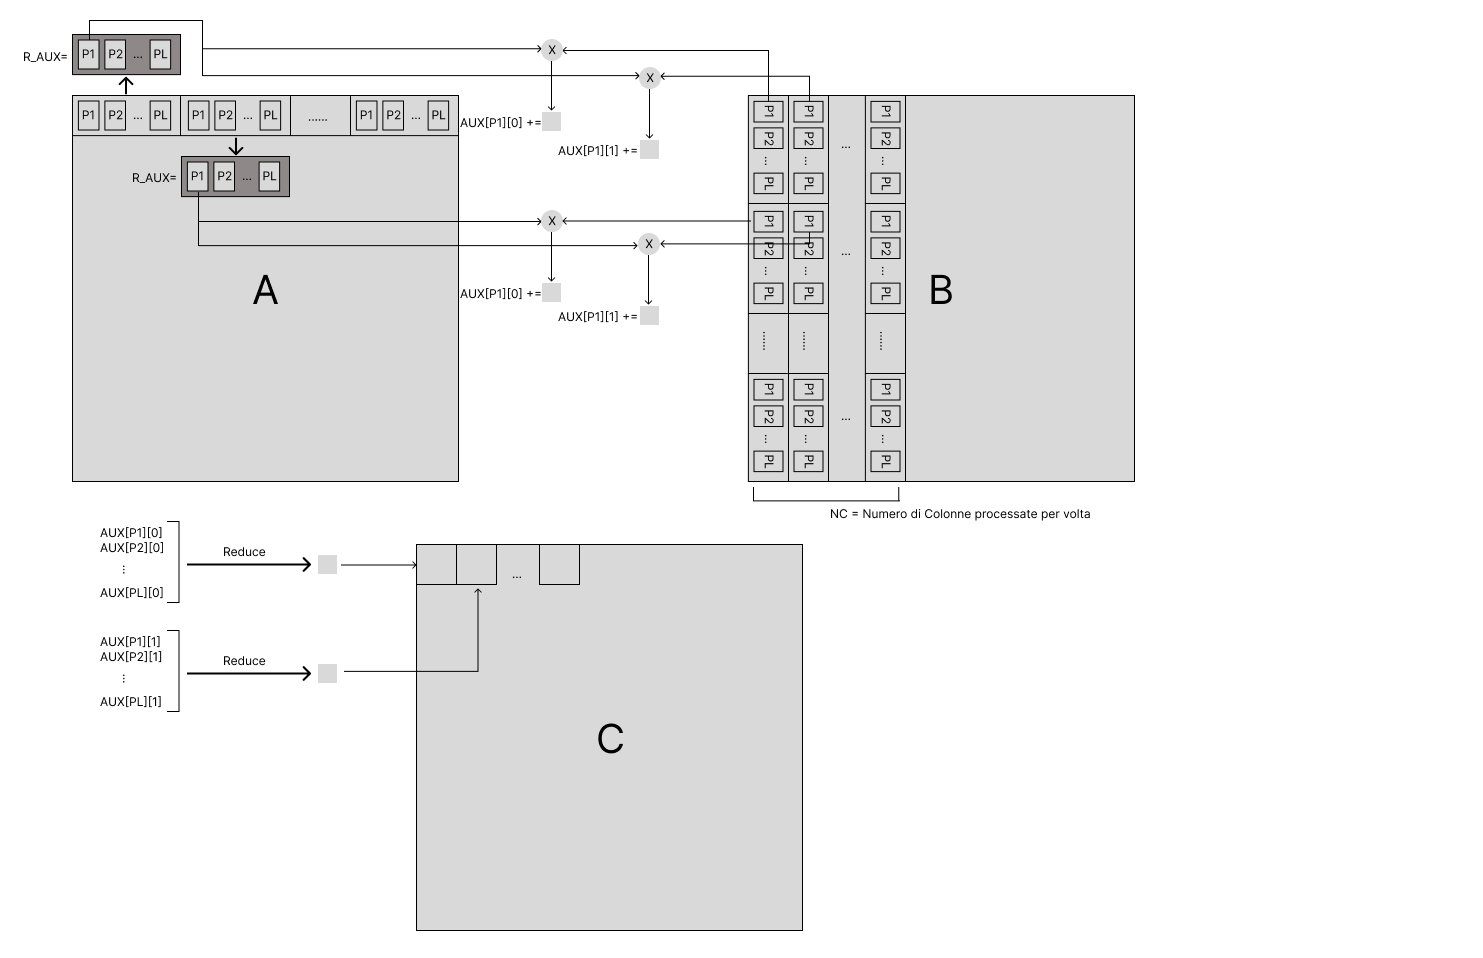
\includegraphics[width=1.1\textwidth]{resources/cuda_scheme_v3.png}
            \end{adjustbox}
        \end{minipage}
        
    \end{columns}
\end{frame}
\subsection{Configurazione dei parametri}
\subsubsection*{Thread}
\begin{frame}{\secname \text{ }- \subsecname\ \text{ }- \subsubsecname}
    %TODO
\end{frame}

\subsubsection*{Shared memory}
\begin{frame}{\secname \text{ }- \subsecname\ \text{ }- \subsubsecname}
    %TODO
\end{frame}

\subsubsection*{Bank conflit}
\begin{frame}{\secname \text{ }- \subsecname\ \text{ }- \subsubsecname}
    %TODO
\end{frame}

%---------------------MPI+CUDA------------------------------
\section{MPI+CUDA}

\begin{frame}{\secname}
    %TODO
\end{frame}

%---------------------Analisi delle prestazioni------------------------------
\section{Analisi delle prestazioni}

\subsection{MPI}
\begin{frame}{\secname \text{ }- \subsecname\ }
    %TODO
\end{frame}

\subsubsection*{Matrici quadrate}
\begin{frame}{\secname \text{ }- \subsecname\ \text{ }- \subsubsecname}
    %TODO
\end{frame}

\subsubsection*{Matrici rettangolari}
\begin{frame}{\secname \text{ }- \subsecname\ \text{ }- \subsubsecname}
    %TODO
\end{frame}

\subsection{CUDA}
\begin{frame}{\secname \text{ }- \subsecname\ }
    %TODO
\end{frame}

\subsubsection*{Matrici quadrate}
\begin{frame}{\secname \text{ }- \subsecname\ \text{ }- \subsubsecname}
    %TODO
\end{frame}

\subsubsection*{Matrici rettangolari}
\begin{frame}{\secname \text{ }- \subsecname\ \text{ }- \subsubsecname}
    %TODO
\end{frame}

\subsection{MPI+CUDA}
\begin{frame}{\secname \text{ }- \subsecname\ }
    %TODO
\end{frame}

\subsubsection*{Matrici quadrate}
\begin{frame}{\secname \text{ }- \subsecname\ \text{ }- \subsubsecname}
    %TODO
\end{frame}

\subsubsection*{MPI+CUDA}
\begin{frame}{\secname \text{ }- \subsecname\ \text{ }- \subsubsecname}
    %TODO
\end{frame}


\begin{frame}
    \frametitle{Grazie per l'attenzione!}
    \begin{itemize}
        \item Tutto il codice che implementa il progetto è disponibile al
        seguente repository: \href{https://github.com/LucaFalasca/ParallelMatrixMultiplication}{https://github.com/LucaFalasca/ParallelMatrixMultiplication}
        \item contattaci a:
            \begin{itemize}
                \item \href{mailto:matteo.conti@students.uniroma2.eu}{matteo.conti@students.uniroma2.eu}
                \item \href{mailto:luca.falasca@students.uniroma2.eu}{luca.falasca@students.uniroma2.eu}
            \end{itemize}
       \end{itemize}
\end{frame}


\end{document}
